\section{Formale Definition}
\label{sec:model-definition}

Weil sie fähig sind, zeitliche Zustände zu speichern, eignen sich Rekurrente Neuronale Netze (in der restlichen Arbeit wird die Abkürzung «RNN» verwendet) besonders gut, um Sequenzen zu lernen.
Die natürliche Sprache ist eine Sequenz von Wörtern, die in sich wiederum aus einer Sequenz von Buchstaben bestehen.
Deshalb kommen RNNs bis heute in vielen Gebieten von natürlichsprachlicher Textverarbeitung zum Einsatz.

Die Besonderheit eines RNN's liegt darin, dass – anders als bei einfachen neuronalen Netzen – die \glspl{neuron} nicht nur den Wert der vorangehenden Netzschicht als
Eingangswert erhalten, sondern auch den Ausgangswert des vorangehenden Zeitschritts ihrer selbst.
Jedes \gls{neuron} speichert den Zustand der bisherigen Zeitschritte als sog. «hidden state», der mit der Variable $ h $ gekennzeichnet wird (siehe Abb. \ref{fig:rnn-model-definition-memory-cell}).
Da das Neuron einr Art Erinnerung fähig ist, wird es auch als «Memory Cell» oder einfach als Zelle bezeichnet.
Der Wert der Zellenausgabe $ y $ sowie der Zustand $ h $ werden beide durch eine Funktion $ f(h_{(t-1)}, x_{(t)})$ anhand des Zustandes aus dem vorangehenden Zeitschritt sowie der Eingabe berechnet.
Die beiden Funktionen können, müssen aber nicht den gleichen Wert ausgeben.
Für nähere Details zur Architektur und Funktionsweise sei auf die exzellente Beschreibung in \autocite{geron} verwiesen.

\begin{figure}
    \centering
    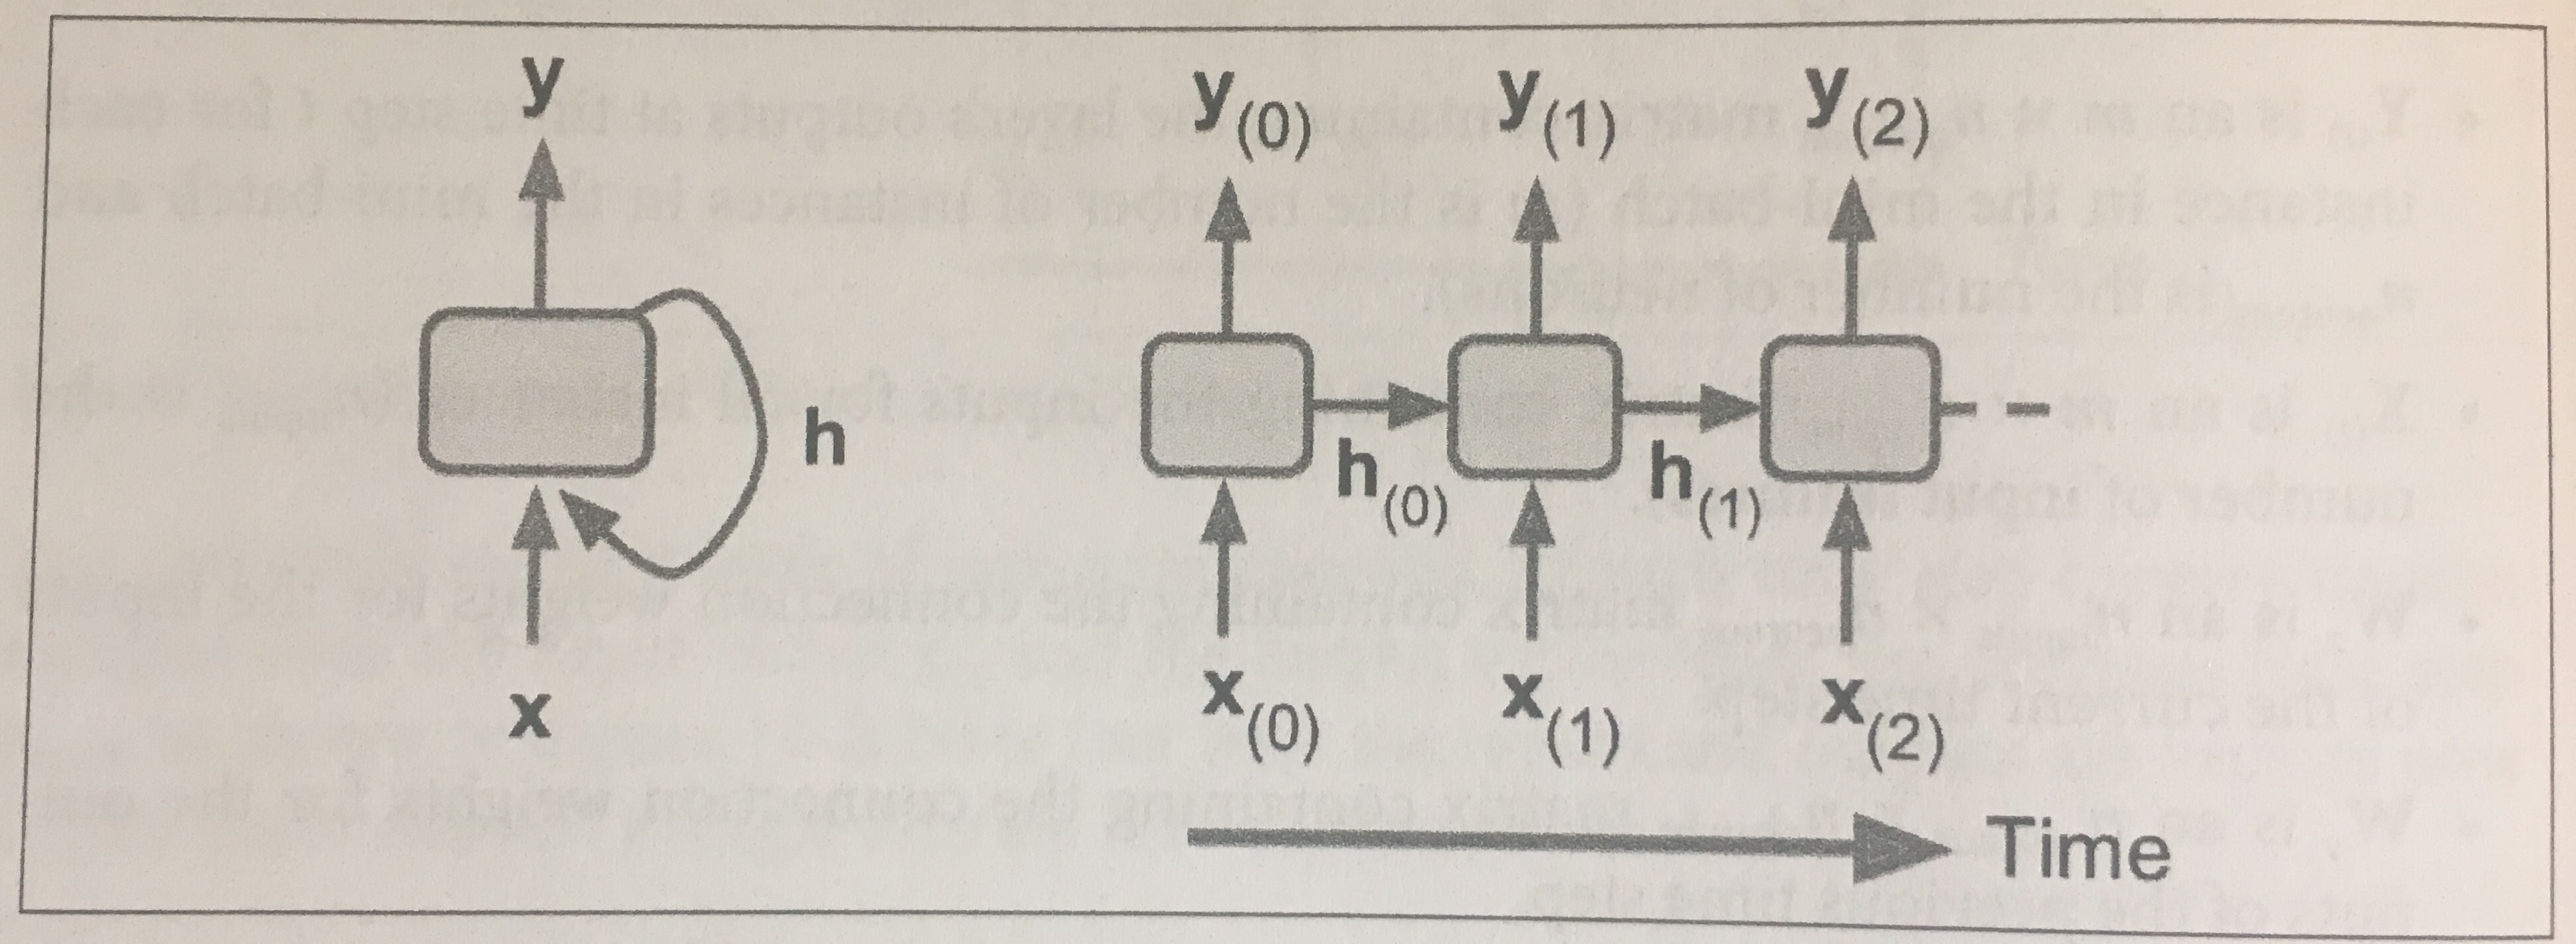
\includegraphics[width=0.75\linewidth]{images/model/model-rnn-definition.jpg}
    \caption[RNN Modell]{Memory-Zelle eines RNN \autocite{geron}}
    \label{fig:rnn-model-definition-memory-cell}
\end{figure}

Zwei gut bekannte Probleme, die einfache RNN-Memory-Zellen aufweisen sind einerseits das sog. «Exploding/Vanishing Gradient Problem», bei dem insbesondere in mehrschichtigen neuronalen Netzen
die propagierten Werte «explodieren» oder gegen null «verschwinden», andererseits das Problem, dass anfangs eingespeiste Informationen gegen Ende der Sequenz verloren gehen \autocite{geron}.
Zur Lösung dieser Problem wurden sog. «Long-Short-Term Memory Cells» (LSTM)\autocite{lstm} und später sog. «Gated Recurrent Units» (GRU)\autocite{gru} entwickelt.
Weil sich beide «Gedächtniszellen» als sehr erfolgreich bewiesen haben, werden einfache RNN-Zellen schon fast nicht mehr verwendet.

Für das hier angewandte Modell sollen LSTMs verwendet werden.
Eine Trainingssequenz (1) wird Buchstabe um Buchstabe in das Modell eingegeben.
Weil Buchstaben an sich nicht für arithmetische Operationen innerhalb des RNNs verwendet werden können, werden sie V-dimensionale One-hot-Vektoren encodiert, wobei die Konstante $ V $ die Menge des Vokabulars darstellt (2).
Das RNN besteht aus einer oder mehreren Schichten (3).
Eine RNN-Zelle besteht wiederum aus einer bestimmten Anzahl an Neuronen oder «Units» (4).
Nachdem die ganze Buchstabensequenz ins RNN eingegeben wurde, wird der letzte Ausgabe-Vektor der LSTM-Zelle ($ y_{1,t} $) durch einen Softmax-Layer auf den Wertebereich (0.0, …, 1.0) normalisiert (5).
So stellt der Ausgabevektor eine Wahrscheinlichkeitsverteilung über das ganze Vokabular dar.
Der Index derjenigen Vektor-Komponente mit der höchsten Wahrscheinlichkeit ist gleichzeitig der Index des vorhergesagten nächsten Buchstanbes in der Sequenz im Vokabular (siehe Abb. \ref{fig:rnn-model-definition}).

\begin{figure}
    \centering
    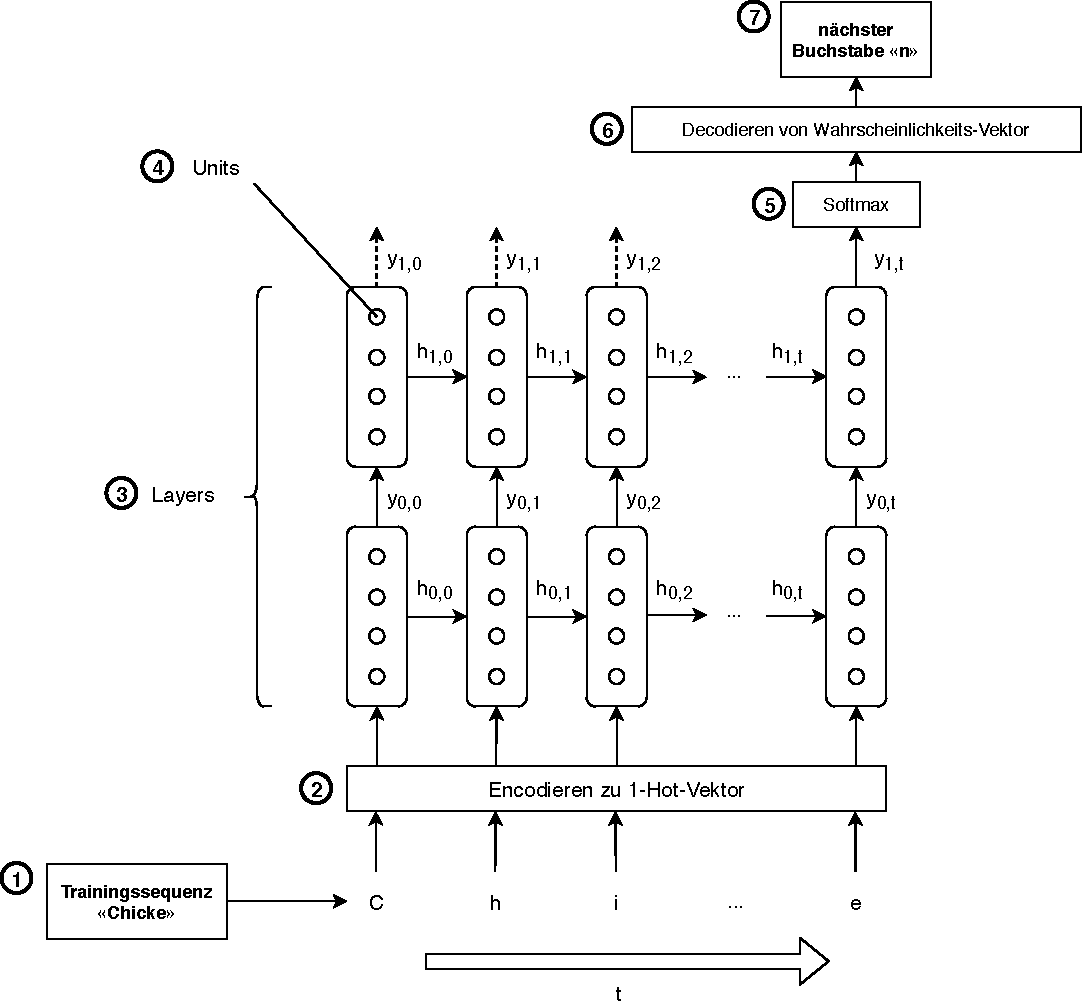
\includegraphics[width=0.9\linewidth]{images/diagrams/model.pdf}
    \caption{RNN Modell}
    \label{fig:rnn-model-definition}
\end{figure}

